\documentclass[11pt,preprint, authoryear]{elsarticle}

\usepackage{lmodern}
%%%% My spacing
\usepackage{setspace}
\setstretch{1.2}
\DeclareMathSizes{12}{14}{10}{10}

% Wrap around which gives all figures included the [H] command, or places it "here". This can be tedious to code in Rmarkdown.
\usepackage{float}
\let\origfigure\figure
\let\endorigfigure\endfigure
\renewenvironment{figure}[1][2] {
    \expandafter\origfigure\expandafter[H]
} {
    \endorigfigure
}

\let\origtable\table
\let\endorigtable\endtable
\renewenvironment{table}[1][2] {
    \expandafter\origtable\expandafter[H]
} {
    \endorigtable
}


\usepackage{ifxetex,ifluatex}
\usepackage{fixltx2e} % provides \textsubscript
\ifnum 0\ifxetex 1\fi\ifluatex 1\fi=0 % if pdftex
  \usepackage[T1]{fontenc}
  \usepackage[utf8]{inputenc}
\else % if luatex or xelatex
  \ifxetex
    \usepackage{mathspec}
    \usepackage{xltxtra,xunicode}
  \else
    \usepackage{fontspec}
  \fi
  \defaultfontfeatures{Mapping=tex-text,Scale=MatchLowercase}
  \newcommand{\euro}{€}
\fi

\usepackage{amssymb, amsmath, amsthm, amsfonts}

\def\bibsection{\section*{References}} %%% Make "References" appear before bibliography


\usepackage[round]{natbib}

\usepackage{longtable}
\usepackage[margin=2.3cm,bottom=2cm,top=2.5cm, includefoot]{geometry}
\usepackage{fancyhdr}
\usepackage[bottom, hang, flushmargin]{footmisc}
\usepackage{graphicx}
\numberwithin{equation}{section}
\numberwithin{figure}{section}
\numberwithin{table}{section}
\setlength{\parindent}{0cm}
\setlength{\parskip}{1.3ex plus 0.5ex minus 0.3ex}
\usepackage{textcomp}
\renewcommand{\headrulewidth}{0.2pt}
\renewcommand{\footrulewidth}{0.3pt}

\usepackage{array}
\newcolumntype{x}[1]{>{\centering\arraybackslash\hspace{0pt}}p{#1}}

%%%%  Remove the "preprint submitted to" part. Don't worry about this either, it just looks better without it:
\makeatletter
\def\ps@pprintTitle{%
  \let\@oddhead\@empty
  \let\@evenhead\@empty
  \let\@oddfoot\@empty
  \let\@evenfoot\@oddfoot
}
\makeatother

 \def\tightlist{} % This allows for subbullets!

\usepackage{hyperref}
\hypersetup{breaklinks=true,
            bookmarks=true,
            colorlinks=true,
            citecolor=blue,
            urlcolor=blue,
            linkcolor=blue,
            pdfborder={0 0 0}}


% The following packages allow huxtable to work:
\usepackage{siunitx}
\usepackage{multirow}
\usepackage{hhline}
\usepackage{calc}
\usepackage{tabularx}
\usepackage{booktabs}
\usepackage{caption}


\newenvironment{columns}[1][]{}{}

\newenvironment{column}[1]{\begin{minipage}{#1}\ignorespaces}{%
\end{minipage}
\ifhmode\unskip\fi
\aftergroup\useignorespacesandallpars}

\def\useignorespacesandallpars#1\ignorespaces\fi{%
#1\fi\ignorespacesandallpars}

\makeatletter
\def\ignorespacesandallpars{%
  \@ifnextchar\par
    {\expandafter\ignorespacesandallpars\@gobble}%
    {}%
}
\makeatother

\newenvironment{CSLReferences}[2]{%
}

\urlstyle{same}  % don't use monospace font for urls
\setlength{\parindent}{0pt}
\setlength{\parskip}{6pt plus 2pt minus 1pt}
\setlength{\emergencystretch}{3em}  % prevent overfull lines
\setcounter{secnumdepth}{5}

%%% Use protect on footnotes to avoid problems with footnotes in titles
\let\rmarkdownfootnote\footnote%
\def\footnote{\protect\rmarkdownfootnote}
\IfFileExists{upquote.sty}{\usepackage{upquote}}{}

%%% Include extra packages specified by user

%%% Hard setting column skips for reports - this ensures greater consistency and control over the length settings in the document.
%% page layout
%% paragraphs
\setlength{\baselineskip}{12pt plus 0pt minus 0pt}
\setlength{\parskip}{12pt plus 0pt minus 0pt}
\setlength{\parindent}{0pt plus 0pt minus 0pt}
%% floats
\setlength{\floatsep}{12pt plus 0 pt minus 0pt}
\setlength{\textfloatsep}{20pt plus 0pt minus 0pt}
\setlength{\intextsep}{14pt plus 0pt minus 0pt}
\setlength{\dbltextfloatsep}{20pt plus 0pt minus 0pt}
\setlength{\dblfloatsep}{14pt plus 0pt minus 0pt}
%% maths
\setlength{\abovedisplayskip}{12pt plus 0pt minus 0pt}
\setlength{\belowdisplayskip}{12pt plus 0pt minus 0pt}
%% lists
\setlength{\topsep}{10pt plus 0pt minus 0pt}
\setlength{\partopsep}{3pt plus 0pt minus 0pt}
\setlength{\itemsep}{5pt plus 0pt minus 0pt}
\setlength{\labelsep}{8mm plus 0mm minus 0mm}
\setlength{\parsep}{\the\parskip}
\setlength{\listparindent}{\the\parindent}
%% verbatim
\setlength{\fboxsep}{5pt plus 0pt minus 0pt}



\begin{document}



\begin{frontmatter}  %

\title{22581340\_Apps}

% Set to FALSE if wanting to remove title (for submission)




\author[Add1]{Gabriella Neilon}
\ead{22581340@sun.ac.za}





\address[Add1]{Stellenbosch University}

\cortext[cor]{Corresponding author: Gabriella Neilon}

\begin{abstract}
\small{
In this report, I explored various aspects of mobile apps, including
their earnings, user reviews, and sentiment analysis. I investigated the
relationship between app categories, earnings, and user sentiment to
gain insights into their interplay. Additionally, I examined the
limitations and potential biases associated with relying solely on user
reviews as a metric for app success.
}
\end{abstract}

\vspace{1cm}





\vspace{0.5cm}

\end{frontmatter}

\setcounter{footnote}{0}



%________________________
% Header and Footers
%%%%%%%%%%%%%%%%%%%%%%%%%%%%%%%%%
\pagestyle{fancy}
\chead{}
\rhead{}
\lfoot{}
\rfoot{\footnotesize Page \thepage}
\lhead{}
%\rfoot{\footnotesize Page \thepage } % "e.g. Page 2"
\cfoot{}

%\setlength\headheight{30pt}
%%%%%%%%%%%%%%%%%%%%%%%%%%%%%%%%%
%________________________

\headsep 35pt % So that header does not go over title




\hypertarget{introduction}{%
\section{\texorpdfstring{Introduction
\label{Introduction}}{Introduction }}\label{introduction}}

Mobile apps have become an integral part of our daily lives, offering a
wide range of functionalities and entertainment options. Understanding
the dynamics between app categories, earnings, and user sentiments is
crucial for app developers, marketers, and decision-makers. In this
analysis, I delve into the characteristics of different app categories
and their implications for earnings and user reviews.

\hypertarget{part-a}{%
\section{Part A}\label{part-a}}

Plotting Earnings by Category and Rating

Through an analysis of the apps data, I explore the relationship between
app categories, ratings, and their respective earnings. The purpose of
this analysis is to determine if ratings play a significant role in
determining app earnings and to identify the top-earning categories.

The findings reveal an intriguing insight: ratings do not seem to be the
sole determining factor for app earnings. Instead, we observe that
certain app categories consistently outperform others in terms of
earnings.

The top five app categories that exhibit the highest earnings are
Family, Lifestyle, Finance, Games, and Photography. This information can
be invaluable for developers, investors, and industry professionals
seeking to make informed decisions about app development and
monetization strategies.

Overall, this analysis highlights the significance of app category
selection and the potential impact it can have on earnings. While
ratings may influence user perception and adoption, it is ultimately the
app category that plays a pivotal role in determining financial success.

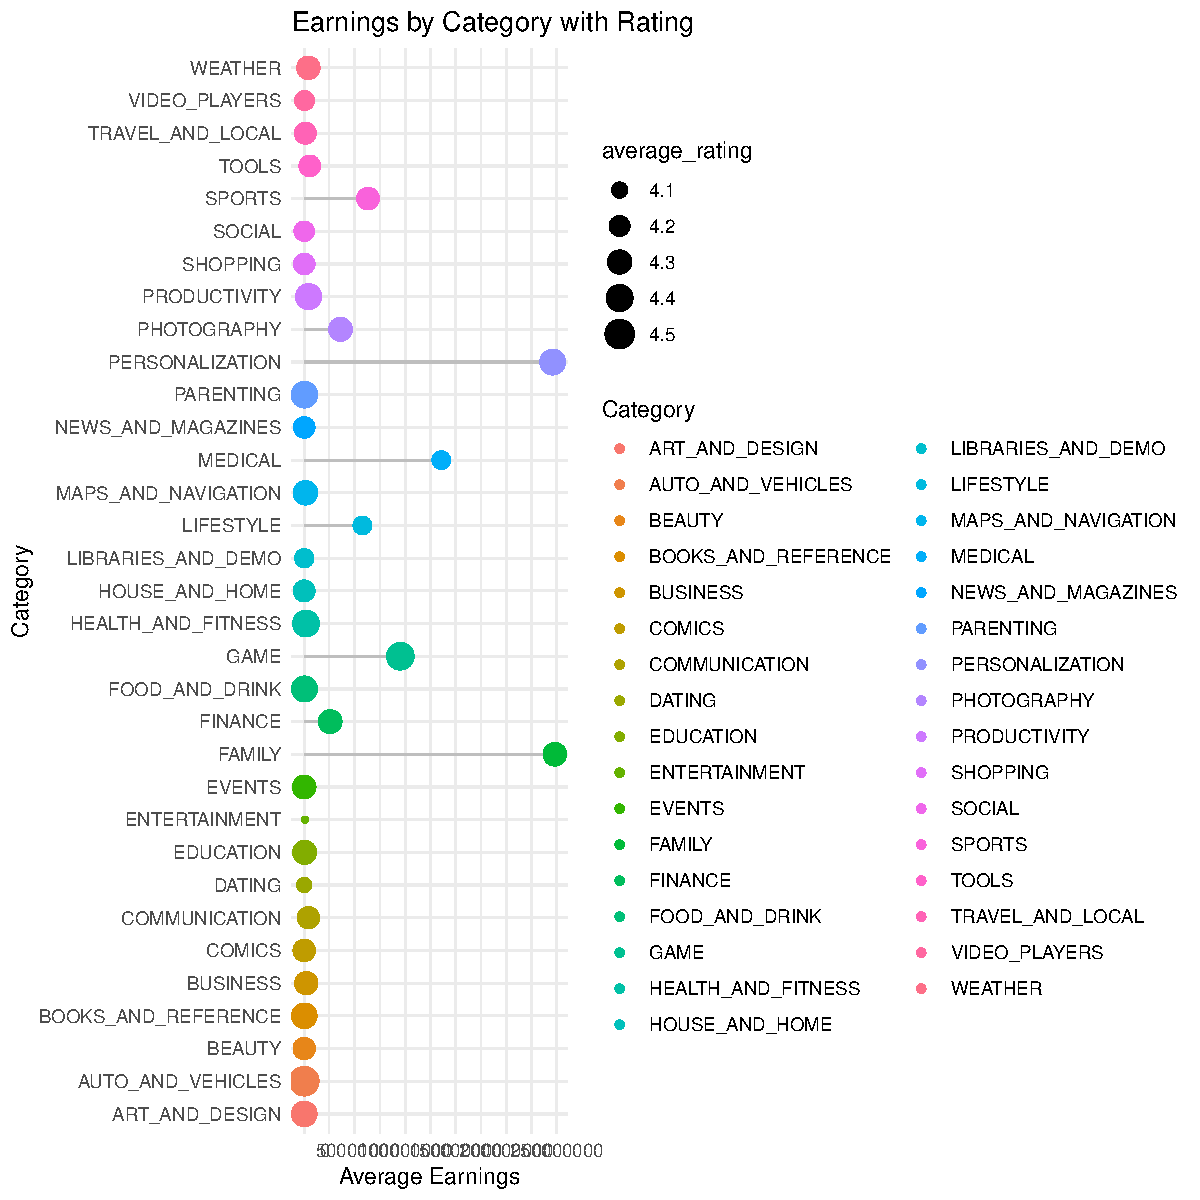
\includegraphics[angle=90]{Question5_files/figure-latex/unnamed-chunk-1-1}

\hypertarget{part-b}{%
\section{Part B}\label{part-b}}

Analysis of Sentiments and Reviews by Category

In this section, I delve into the sentiments expressed in customer
reviews for the top five categories identified in the previous section.
The analysis aims to shed light on the prevalence of positive, negative,
and neutral sentiments within each category, providing insights into
customer perceptions and experiences.

To begin, I quantify the number of positive, negative, and neutral
sentiments for each category. This initial step allows us to understand
the sentiment distribution and identify any significant patterns or
variations across categories. Next, I explore the total number of
reviews for each category. By considering the overall review volume, we
gain a sense of the level of customer engagement and interest within
each category. To gain a more comprehensive understanding, I calculate
the percentage of positive, negative, and neutral reviews for each
category by dividing the sentiments by the total reviews. This
normalization allows us to compare sentiments across categories,
considering the differences in review volume.

Based on the calculated percentages, I present a table that showcases
the distribution of positive, neutral, and negative reviews as a
percentage of the total reviews for each category. This table provides a
concise overview of the sentiment composition within each category.

Despite Photography being the category with the least earnings among the
five categories (Lifestyle, Family, Game, Finance, and Photography), it
surprisingly receives the highest number of positive reviews. This
finding suggests that relying solely on reviews as a metric may not be a
reliable indicator for predicting prospective earnings. Other factors
such as user preferences, marketing strategies, and market demand may
play significant roles in determining the success of an app within a
particular category.

\begin{longtable}[]{@{}lllrrr@{}}
\caption{App Sentiment}\tabularnewline
\toprule()
& Category & Sentiment & Count & Total & Percentage \\
\midrule()
\endfirsthead
\toprule()
& Category & Sentiment & Count & Total & Percentage \\
\midrule()
\endhead
1 & FAMILY & Negative & 886 & 3440 & 25.755814 \\
2 & FAMILY & Neutral & 361 & 3440 & 10.494186 \\
3 & FAMILY & Positive & 2193 & 3440 & 63.750000 \\
4 & FINANCE & Negative & 322 & 1491 & 21.596244 \\
5 & FINANCE & Neutral & 217 & 1491 & 14.553991 \\
6 & FINANCE & Positive & 952 & 1491 & 63.849765 \\
7 & GAME & Negative & 2493 & 6643 & 37.528225 \\
8 & GAME & Neutral & 290 & 6643 & 4.365498 \\
9 & GAME & Positive & 3860 & 6643 & 58.106277 \\
10 & LIFESTYLE & Negative & 235 & 1196 & 19.648829 \\
11 & LIFESTYLE & Neutral & 266 & 1196 & 22.240803 \\
12 & LIFESTYLE & Positive & 695 & 1196 & 58.110368 \\
13 & PHOTOGRAPHY & Negative & 254 & 1245 & 20.401606 \\
14 & PHOTOGRAPHY & Neutral & 173 & 1245 & 13.895582 \\
15 & PHOTOGRAPHY & Positive & 818 & 1245 & 65.702811 \\
\bottomrule()
\end{longtable}

\hfill

\hypertarget{conclusion}{%
\section{Conclusion}\label{conclusion}}

The relationship between app categories, earnings, and user sentiment is
complex and multifaceted. While positive reviews generally dominate
across different app categories, it is crucial to consider additional
factors such as user preferences, marketing strategies, and market
demand when assessing the potential success of an app. A prime example
is the category ``Photography'', it had relatively lower earnings
compared to other categories, but it surprisingly received the highest
number of positive reviews. This discrepancy highlights the limitations
of using user reviews as a sole metric for determining app success, as
factors beyond reviews may influence the earnings potential of an app.

\bibliography{Tex/ref}





\end{document}
